\documentclass[letterpaper,12pt]{article}
\usepackage{array}
\usepackage{threeparttable}
\usepackage{geometry}
\geometry{letterpaper,tmargin=1in,bmargin=1in,lmargin=1.25in,rmargin=1.25in}
\usepackage{fancyhdr,lastpage}
\pagestyle{fancy}
\lhead{}
\chead{}
\rhead{}
\lfoot{}
\cfoot{}
\rfoot{\footnotesize\textsl{Page \thepage\ of \pageref{LastPage}}}
\renewcommand\headrulewidth{0pt}
\renewcommand\footrulewidth{0pt}
\usepackage[format=hang,font=normalsize,labelfont=bf]{caption}
\usepackage{listings}
\lstset{frame=single,
  language=Python,
  showstringspaces=false,
  columns=flexible,
  basicstyle={\small\ttfamily},
  numbers=none,
  breaklines=true,
  breakatwhitespace=true
  tabsize=3
}
\usepackage{amsmath}
\usepackage{amssymb}
\usepackage{amsthm}
\usepackage{harvard}
\usepackage{setspace}
\usepackage{float,color}
\usepackage[pdftex]{graphicx}
\usepackage{hyperref}
\hypersetup{colorlinks,linkcolor=red,urlcolor=blue}
\theoremstyle{definition}
\newtheorem{theorem}{Theorem}
\newtheorem{acknowledgement}[theorem]{Acknowledgement}
\newtheorem{algorithm}[theorem]{Algorithm}
\newtheorem{axiom}[theorem]{Axiom}
\newtheorem{case}[theorem]{Case}
\newtheorem{claim}[theorem]{Claim}
\newtheorem{conclusion}[theorem]{Conclusion}
\newtheorem{condition}[theorem]{Condition}
\newtheorem{conjecture}[theorem]{Conjecture}
\newtheorem{corollary}[theorem]{Corollary}
\newtheorem{criterion}[theorem]{Criterion}
\newtheorem{definition}[theorem]{Definition}
\newtheorem{derivation}{Derivation} % Number derivations on their own
\newtheorem{example}[theorem]{Example}
\newtheorem{exercise}[theorem]{Exercise}
\newtheorem{lemma}[theorem]{Lemma}
\newtheorem{notation}[theorem]{Notation}
\newtheorem{problem}[theorem]{Problem}
\newtheorem{proposition}{Proposition} % Number propositions on their own
\newtheorem{remark}[theorem]{Remark}
\newtheorem{solution}[theorem]{Solution}
\newtheorem{summary}[theorem]{Summary}
%\numberwithin{equation}{section}
\bibliographystyle{aer}
\newcommand\ve{\varepsilon}
\newcommand\boldline{\arrayrulewidth{1pt}\hline}


\begin{document}

\begin{flushleft}
  \textbf{\large{Econ Problem Set \#1}} \\
  Charlie Walker
\end{flushleft}

\vspace{5mm}

\noindent\textbf{Problem 1}\\
$\{\overline{b}_s\}_{s=1}^3 = [0.01931, 0.05861]$\\
$\{\overline{c}_s\}_{s=1}^3 = [0.18241, 0.34384, 0.24087]$\\
$\overline{w} = 0.2017$\\
$\overline{r} = 2.4330$\\


\noindent\textbf{Problem 2}\\
With $\beta = 0.55$, the new steady-state is:\newline\\
$\{\overline{b}_s\}_{s=1}^3 = [0.02817, 0.07686]$\\
$\{\overline{c}_s\}_{s=1}^3 = [0.19597, 0.36915, 0.26669]$\\
$\overline{w} = 0.22415$\\
$\overline{r} = 1.88636$\newline\\
As households become more patient, savings increase, consumption increases uniformly across a lifetime, wages are higher, and interest rates are lower. Savings are higher as a result of households' increased patience; this leads to a larger capital stock, pushing down interest rates. \\

\noindent\textbf{Problem 3/4}\\
Figure 1 plots the equilibrium time path of the aggregate capital stock $\{K_t\}_{t=1}^{15}$. It took the economy 8 periods to get within 0.0001 of the steady-state aggregate capital stock, $\overline{K}=0.07772$ (this ignores the fluctuations from $t=1$ to $t=5$ that can be seen in the plot).
\begin{figure}[htb]\centering\captionsetup{width=4.0in}
  \caption{\textbf{Equilibrium Capital Time Path}}\label{FigExample}
  \fbox{\resizebox{4.0in}{3.0in}{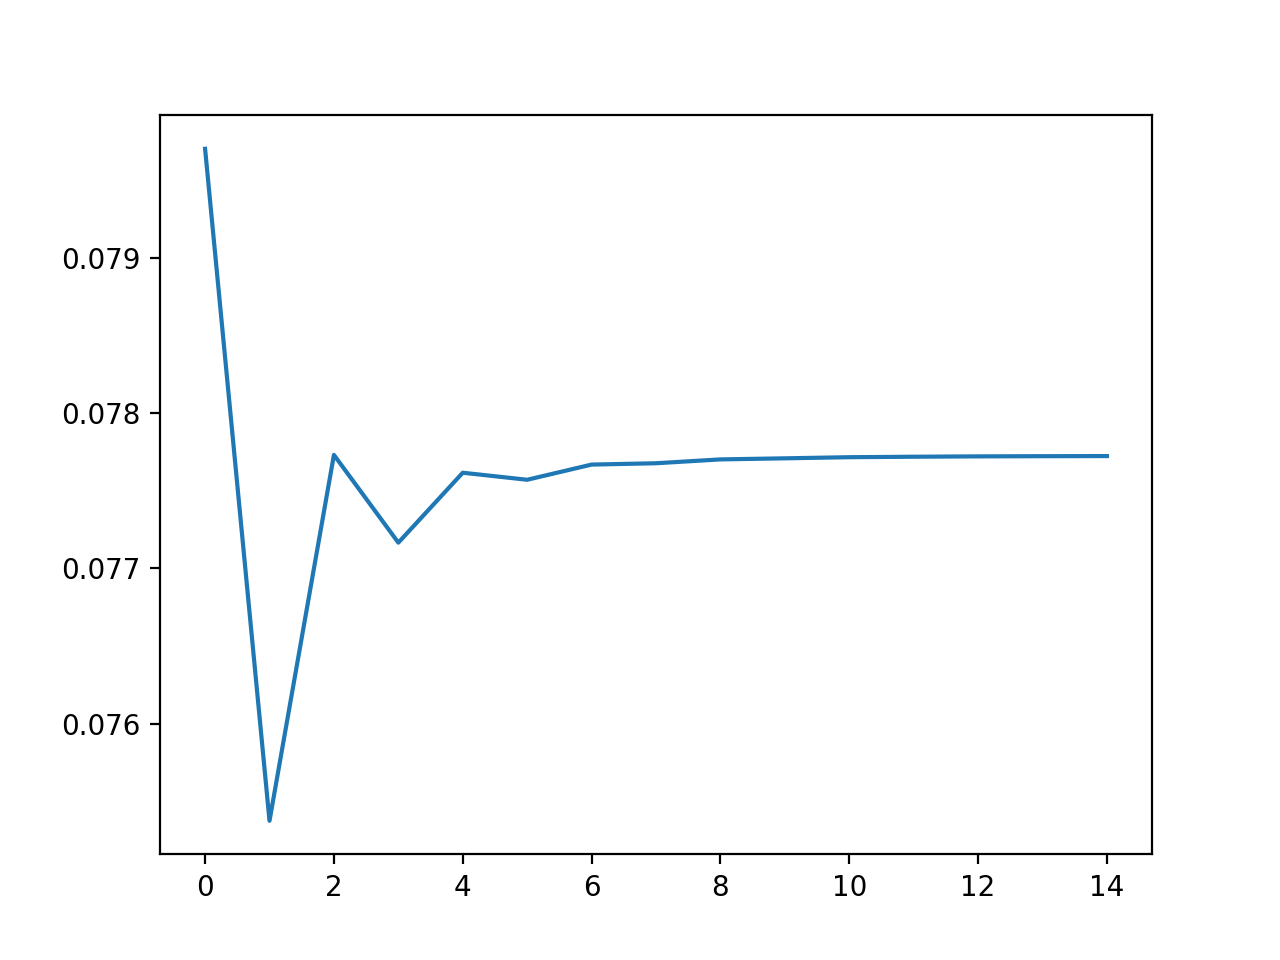
\includegraphics{figure_1.png}}}
\end{figure}



\end{document}

